%% LyX 2.0.6 created this file.  For more info, see http://www.lyx.org/.
%% Do not edit unless you really know what you are doing.
\documentclass[a4paper,english]{article}
\usepackage{babel}
\usepackage{amsmath}
\usepackage{graphicx}
\usepackage[unicode=true,
 bookmarks=true,bookmarksnumbered=false,bookmarksopen=false,
 breaklinks=false,pdfborder={0 0 1},backref=false,colorlinks=false]
 {hyperref}
\hypersetup{pdftitle={LyTeX},
 pdfauthor={Jiangbing},
 pdfsubject={latex},
 unicode=false}

\makeatletter

%%%%%%%%%%%%%%%%%%%%%%%%%%%%%% LyX specific LaTeX commands.
\pdfpageheight\paperheight
\pdfpagewidth\paperwidth

%% Because html converters don't know tabularnewline
\providecommand{\tabularnewline}{\\}

%%%%%%%%%%%%%%%%%%%%%%%%%%%%%% User specified LaTeX commands.
% please do NOT remove these lines!
% set file encoding for WinEdt
% !Mode:: "TeX:UTF-8"
% set typesetting program for TeXworks
% !TEX program = XeLaTeX

\usepackage[CJKtextspaces,CJKnumber]{xeCJK}                                      
\setCJKmainfont[BoldFont=SimHei]{SimSun}
\setCJKsansfont{SimHei}         
\setCJKmonofont{NSimSun}  

\setCJKfamilyfont{song}{SimSun}
\setCJKfamilyfont{hei}{SimHei}

\makeatother

\usepackage{xunicode}
\begin{document}

\title{多元回归的学习与简单总结}


\author{蒋冰\date{}}

\maketitle
\begin{center}
学号:201322130002
\par\end{center}
\begin{abstract}
本文由问题引入,简单介绍多元线性回归模型及其参数的求解,然后用多元线性回归模型来测算糖尿病患者的血清总胆固醇、甘油三酯、空腹胰岛素、糖化血红蛋白和空腹血糖的测量值之间的关系。然后进行了方差分析,根据F检验求得的统计量确定所建的回归方程具有统计学意义。而且回归模型的$R^{2}=0.6008$说明模型拟合结果较好,但仍希望能进一步提高拟合效果。于是做了t检验分析各项回归系数的显著性并求了回归系数的置信区间。由标准化回归方程和偏回归平方和可以比较各项变量对因变量的影响。考虑到回归系数可能受到其他变量的影响,又做了自变量的选择和是否存在交互作用的判断。为判断回归模型时候有效,本文又比较了回归的残差并检验了其正态性,而且检验得回归的设计矩阵的多重共线性很小。为比较普通最小二乘法的效果,本文又比较了岭回归和主成分分析做出的回归方程。

通过多元线性回归模型的实际应用,本文谈论了多元线性回归的应用的应用场景和作用,证实了多元线性回归具有很重要的实际意义。
\end{abstract}

\section{多元线性回归模型介绍}


\subsection{问题引入}

回归分析是利用大量的观测数据来确定变量与变量之间的统计相关关系的一种数理统计方法。

由于事物间的联系常常是多方面的,一个因变量的变化可能受到其它多个自变量的影响,如糖尿病患者的血糖变化可能受胰岛素、糖化血红蛋白、血清总胆固醇、甘油三脂等多种生化指标的影响。因此,多元回归分析,作为一种以多个自变量估计因变量的线性关系的方法,常常被用来解释和预报因变量的变化。


\subsection{多元线性回归模型介绍}

在多元回归分析中,因变量只有1个,常用变量$Y$表示,自变量往往不止1个,通常设为m个($m\geq2$),分别记作$X_{1},X_{2},\cdots,X_{m}$,共m+1个变量。设观测样本含量为n。观测数据格式如下图所示:

\begin{tabular}{|c|c|c|c|c|c|}
\hline 
序号i & $X_{1}$ & $X_{2}$ & \ldots{} & $X_{m}$ & $Y$\tabularnewline
\hline 
\hline 
1 & $X_{11}$ & $X_{12}$ & \ldots{} & $X_{1m}$ & $Y_{1}$\tabularnewline
\hline 
2 & $X_{21}$ & $X_{22}$ & \ldots{} & $X_{2m}$ & $Y_{2}$\tabularnewline
\hline 
$\vdots$ & $\vdots$ & $\vdots$ &  & $\vdots$ & $\vdots$\tabularnewline
\hline 
n & $X_{n1}$ & $X_{n1}$ & ··· & $X_{nm}$ & $Y_{n}$\tabularnewline
\hline 
\end{tabular}

假设条件:
\begin{enumerate}
\item Y与$X_{1},X_{2},\cdots,X_{m}$之间具有线性关系。
\item 各例观测值$Y_{i}(i=1,2,\cdots,n)$相互独立。
\item 残差$\varepsilon$服从均值为0,方差为$\sigma^{2}$的正态分布,它等价于对任意一组自变量$X_{1},X_{2},\cdots,X_{m}$的值,因变量$Y$具有相同方差,并且服从正态分布。
\end{enumerate}
回归模型的一般形式如下所示:$Y=\beta_{0}+\beta_{1}X_{1}+\beta_{2}X_{2}+\cdots+\beta_{m}X_{m}+\varepsilon$。式子的含义为数据中因变量$Y$可以近似地表示为自变量$X_{1},X_{2},\cdots,X_{m}$的线性函数。$\beta_{0}$为常数项,$\beta_{1},\beta_{2},\cdots,\beta_{m}$为偏回归系数,表示在其它自变量保持不变时,$X_{j}$增加或减少一个单位时$Y$的平均变
化量,$\varepsilon$是去除m个自变量对Y影响后的随机误差(残差)。


\subsection{多元线性回归系数的最小二乘估计}

设$\hat{\beta_{0}},\hat{\beta_{1}},\hat{\beta_{2}},\cdots,\hat{\beta_{m}}$为$\beta_{0},\beta_{1},\beta_{2},\cdots,\beta_{m}$的最小二乘估计,则y的n次观测值可写为如下形式:

$\begin{cases}
Y_{1}=\hat{\beta_{0}}+\hat{\beta_{1}}X_{11}+\hat{\beta_{2}}X_{12}+\cdots+\hat{\beta_{m}}X_{1m}+\hat{\varepsilon_{1}}\\
Y_{2}=\hat{\beta_{0}}+\hat{\beta_{1}}X_{21}+\hat{\beta_{2}}X_{22}+\cdots+\hat{\beta_{m}}X_{2m}+\hat{\varepsilon_{2}}\\
\cdots\\
Y_{n}=\hat{\beta_{0}}+\hat{\beta_{1}}X_{n1}+\hat{\beta_{2}}X_{n2}+\cdots+\hat{\beta_{m}}X_{nm}+\hat{\varepsilon_{n}}
\end{cases}$

其中$\beta_{1},\beta_{2},\cdots,\beta_{m}$ 是未知参数。其中\foreignlanguage{english}{$\hat{\varepsilon_{i}}$为误差$\varepsilon_{i}$的估计值,称为残差。}

采用矩阵形式可以设

$Y=\left[\begin{array}{c}
y_{1}\\
y_{2}\\
\vdots\\
y_{n}
\end{array}\right]$,$\beta=\left[\begin{array}{c}
\beta_{1}\\
\beta_{2}\\
\vdots\\
\beta_{n}
\end{array}\right]$,$X=\left[\begin{array}{ccccc}
1 & x_{11} & x_{12} & \cdots & x_{1m}\\
1 & x_{21} & x_{22} & \cdots & x_{2m}\\
\vdots & \vdots & \vdots &  & \vdots\\
1 & x_{n1} & x_{n2} & \cdots & x_{nm}
\end{array}\right]$,$\varepsilon=\left[\begin{array}{c}
\varepsilon_{1}\\
\varepsilon_{2}\\
\vdots\\
\varepsilon_{n}
\end{array}\right]$,

则多元模型可以表示为矩阵形式$Y=X\beta+\varepsilon$

令$\hat{Y}$为$Y$的估计值,则有$\hat{Y_{i}}=\hat{\beta_{0}}+\hat{\beta_{1}}X_{i1}+\hat{\beta_{2}}X_{i2}+\cdots+\hat{\beta_{m}}X_{im}$,\foreignlanguage{english}{$\hat{\varepsilon_{i}}=Y_{i}-\hat{Y_{i}}$,为使得估计值与实际值拟合的最好,则应使残差平方和$Q(\hat{\beta_{1}},\hat{\beta_{2}},\cdots,\hat{\beta_{m}})={\displaystyle \sum_{i=1}^{n}\varepsilon_{i}^{2}={\displaystyle \sum_{i=1}^{n}(Y_{i}-\hat{Y_{i}})^{2}={\displaystyle \sum_{i=1}^{n}[Y_{i}-(\hat{\beta_{0}}+\hat{\beta_{1}}X_{i1}+\hat{\beta_{2}}X_{i2}+\cdots+\hat{\beta_{m}}X_{im})]^{2}}}}$达到最小。用矩阵形式表达就是}求使得残差平方和$||\varepsilon||^{2}=\varepsilon^{T}\varepsilon=\left(Y-X\beta\right)^{2}\left(Y-X\beta\right)$达到最小的$\beta$值。\foreignlanguage{english}{因此,对上式对}$\hat{\beta_{0}},\hat{\beta_{1}},\hat{\beta_{2}},\cdots,\hat{\beta_{m}}$分别求导有:

$\begin{cases}
\frac{\partial Q}{\partial\beta_{0}}=-2{\displaystyle \sum_{i=1}^{n}}(Y_{i}-\hat{Y_{i}})=0\\
\frac{\partial Q}{\partial\beta_{j}}=-2{\displaystyle \sum_{i=1}^{n}}(Y_{i}-\hat{Y_{i}})X_{ij}=0 & j=1,2,\cdots,m
\end{cases}$

即$\begin{cases}
{\displaystyle \sum_{i=1}^{n}}(Y_{i}-\hat{\beta_{0}}-\hat{\beta_{1}}X_{i1}-\hat{\beta_{2}}X_{i2}-\cdots-\hat{\beta_{m}}X_{im})=0\\
{\displaystyle \sum_{i=1}^{n}}(Y_{i}-\hat{\beta_{0}}-\hat{\beta_{1}}X_{i1}-\hat{\beta_{2}}X_{i2}-\cdots-\hat{\beta_{m}}X_{im})X_{ij}=0 & j=1,2,\cdots,m
\end{cases}$

整理并化简则得到下列的正规方程组

$\begin{cases}
n\beta_{0}+({\displaystyle \sum_{i=1}^{n}}X_{i1})\hat{\beta_{1}}+({\displaystyle \sum_{i=1}^{n}}X_{i2})\hat{\beta_{2}}+\cdots+({\displaystyle \sum_{i=1}^{n}}X_{im})\hat{\beta_{m}}={\displaystyle \sum_{i=1}^{n}}Y_{i}\\
({\displaystyle \sum_{i=1}^{n}}X_{i1})\beta_{0}+({\displaystyle \sum_{i=1}^{n}}X_{i1}^{2})\hat{\beta_{1}}+({\displaystyle \sum_{i=1}^{n}}X_{i1}X_{i2})\hat{\beta_{2}}+\cdots+({\displaystyle \sum_{i=1}^{n}}X_{i1}X_{im})\hat{\beta_{m}}={\displaystyle \sum_{i=1}^{n}}X_{i1}Y_{i}\\
\cdots\\
({\displaystyle \sum_{i=1}^{n}}X_{im})\beta_{0}+({\displaystyle \sum_{i=1}^{n}}X_{i1}X_{im})\hat{\beta_{1}}+({\displaystyle \sum_{i=1}^{n}}X_{i1}X_{im})\hat{\beta_{2}}+\cdots+({\displaystyle \sum_{i=1}^{n}}X_{im}^{2})\hat{\beta_{m}}={\displaystyle \sum_{i=1}^{n}}X_{im}Y_{i}
\end{cases}$

记方程的系数矩阵为A,常数项矩阵为B,则有

$A=\left[\begin{array}{ccccc}
n & {\displaystyle \sum_{i=1}^{n}}X_{i1} & {\displaystyle \sum_{i=1}^{n}}X_{i2} & \cdots & {\displaystyle \sum_{i=1}^{n}}X_{im}\\
{\displaystyle \sum_{i=1}^{n}}X_{i1} & {\displaystyle \sum_{i=1}^{n}}X_{i1}^{2} & {\displaystyle \sum_{i=1}^{n}}X_{i1}X_{i2} & \cdots & {\displaystyle \sum_{i=1}^{n}}X_{i1}X_{im}\\
\cdots & \cdots & \cdots & \cdots & \cdots\\
{\displaystyle \sum_{i=1}^{n}}X_{im} & {\displaystyle \sum_{i=1}^{n}}X_{i1}X_{im} & {\displaystyle \sum_{i=1}^{n}}X_{i1}X_{im} & \cdots & {\displaystyle \sum_{i=1}^{n}}X_{im}^{2}
\end{array}\right]$

$=\left[\begin{array}{cccc}
1 & 1 & \cdots & 1\\
X_{11} & X_{21} & \cdots & X_{n1}\\
X_{12} & X_{22} & \cdots & X_{n2}\\
\cdots & \cdots & \cdots & \cdots\\
X_{1m} & X_{2m} & \cdots & X_{nm}
\end{array}\right]\left[\begin{array}{ccccc}
1 & X_{11} & X_{12} & \cdots & X_{1m}\\
1 & X_{21} & X_{22} & \cdots & X_{2m}\\
\cdots & \cdots & \cdots & \cdots & \cdots\\
1 & X_{n1} & X_{n2} & \cdots & X_{nm}
\end{array}\right]=X^{T}X$

$B=\left[\begin{array}{c}
{\displaystyle \sum_{i=1}^{n}}Y_{i}\\
{\displaystyle \sum_{i=1}^{n}}X_{i1}Y_{i}\\
\vdots\\
{\displaystyle \sum_{i=1}^{n}}X_{im}Y_{i}
\end{array}\right]=\left[\begin{array}{cccc}
1 & 1 & \cdots & 1\\
X_{11} & X_{21} & \cdots & X_{n1}\\
X_{12} & X_{22} & \cdots & X_{n2}\\
\cdots & \cdots & \cdots & \cdots\\
X_{1m} & X_{2m} & \cdots & X_{nm}
\end{array}\right]\left[\begin{array}{c}
Y_{1}\\
Y_{2}\\
\vdots\\
Y_{n}
\end{array}\right]$

因此正规方程的举证形式为$(X^{T}X)\beta=X^{T}Y$,如果系数矩阵A满秩,则$A^{-1}$存在,此时易求得,$\beta$的最小二乘估计值为$\hat{\beta}=\left(X^{T}X\right)^{-1}X^{T}Y$

从而可得到经验回归方程为:$\hat{Y}=\hat{\beta_{0}}+\hat{\beta_{1}}X_{1}+\hat{\beta_{2}}X_{2}+\cdots+\hat{\beta_{m}}X_{m}$


\section{模型的测算分析}


\subsection{数据来源}

数据为27名糖尿病患者的血清总胆固醇、甘油三酯、空腹胰岛素、糖化血红蛋白和空腹血糖的测量值。数据如下图所示:

\begin{tabular}{|c|c|c|c|c|c|}
\hline 
序号i & $Y$ & $X_{1}$ & $X_{2}$ & $X_{3}$ & $X_{4}$\tabularnewline
\hline 
\hline 
1 & 11.2 & 5.68 & 1.9 & 4.53 & 8.2\tabularnewline
\hline 
2 & 8.8 & 3.79 & 1.64 & 7.32 & 6.9\tabularnewline
\hline 
3 & 12.3 & 6.02 & 3.56 & 6.95 & 10.8\tabularnewline
\hline 
4 & 11.6 & 4.85 & 1.07 & 5.88 & 8.3\tabularnewline
\hline 
5 & 13.4 & 4.6 & 2.32 & 4.05 & 7.5\tabularnewline
\hline 
6 & 18.3 & 6.05 & 0.64 & 1.42 & 13.6\tabularnewline
\hline 
7 & 11.1 & 4.9 & 8.5 & 12.6 & 8.5\tabularnewline
\hline 
8 & 12.1 & 7.08 & 3 & 6.75 & 11.5\tabularnewline
\hline 
9 & 9.6 & 3.85 & 2.11 & 16.28 & 7.9\tabularnewline
\hline 
10 & 8.4 & 4.65 & 0.63 & 6.59 & 7.1\tabularnewline
\hline 
11 & 9.3 & 4.59 & 1.97 & 3.61 & 8.7\tabularnewline
\hline 
12 & 10.6 & 4.29 & 1.97 & 6.61 & 7.8\tabularnewline
\hline 
13 & 8.4 & 7.97 & 1.93 & 7.57 & 9.9\tabularnewline
\hline 
14 & 9.6 & 6.19 & 1.18 & 1.42 & 6.9\tabularnewline
\hline 
15 & 10.9 & 6.13 & 2.06 & 10.35 & 10.5\tabularnewline
\hline 
16 & 10.1 & 5.71 & 1.78 & 8.53 & 8\tabularnewline
\hline 
17 & 14.8 & 6.4 & 2.4 & 4.53 & 10.3\tabularnewline
\hline 
18 & 9.1 & 6.06 & 3.67 & 12.79 & 7.1\tabularnewline
\hline 
19 & 10.8 & 5.09 & 1.03 & 2.53 & 8.9\tabularnewline
\hline 
20 & 10.2 & 6.13 & 1.71 & 5.28 & 9.9\tabularnewline
\hline 
21 & 13.6 & 5.78 & 3.36 & 2.96 & 8\tabularnewline
\hline 
22 & 14.9 & 5.43 & 1.13 & 4.31 & 11.3\tabularnewline
\hline 
23 & 16 & 6.5 & 6.21 & 3.47 & 12.3\tabularnewline
\hline 
24 & 13.2 & 7.98 & 7.92 & 3.37 & 9.8\tabularnewline
\hline 
25 & 20 & 11.54 & 10.89 & 1.2 & 10.5\tabularnewline
\hline 
26 & 13.3 & 5.84 & 0.92 & 8.61 & 6.4\tabularnewline
\hline 
27 & 10.4 & 3.84 & 1.2 & 6.45 & 9.6\tabularnewline
\hline 
\end{tabular}

变量说明如下:

$Y$:空腹血糖的含量(mmol/L);

$X_{1}$:血清总胆固醇的含量(mmol/L);

$X_{2}$:甘油三酯的含量(mmol/L);

$X_{3}$:胰岛素的含量(μ U/L);

$X_{4}$:糖化血红蛋白(\%)。


\subsection{多元线性回归模型及其检验}


\subsubsection{多元线性回归方程}

用R语言,可以求得回归方程为:$\hat{Y}=5.9433+0.1424X_{1}+0.3515X_{2}-0.2706X_{3}+0.6382X_{4}$。从各项系数都为正数可知,糖尿病患者的血清总胆固醇、甘油三酯、空腹胰岛素、糖化血红蛋白都对空腹血糖有着正相关关系,即在其他情况不变的条件下,它们中任何一个升高,对应的平均血糖也会升高。

回归模型的诊断如下图所示:

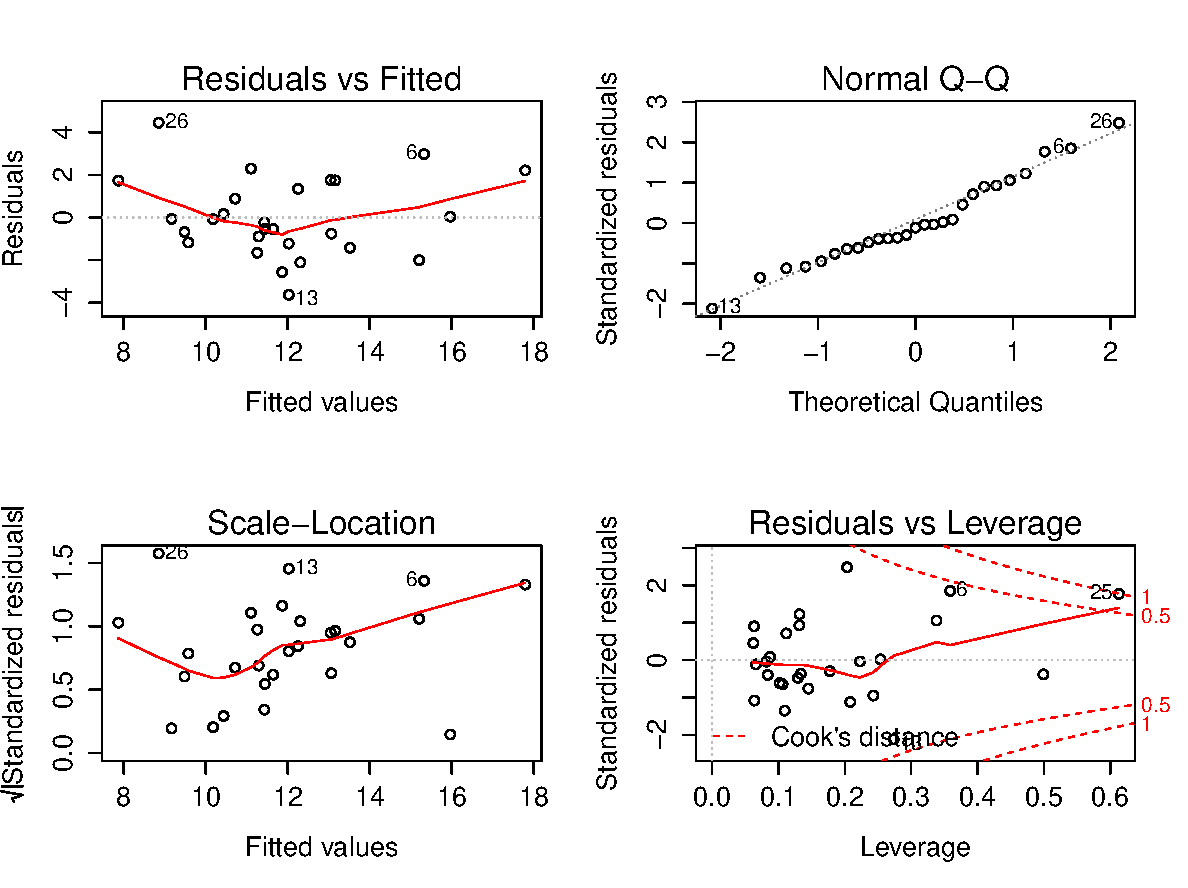
\includegraphics{figure/回归模型诊断1}

如上图所示,回归模型得到的残差较为均匀地分布在零点两侧,没有显示出特定的函数形式。而且通过Q-Q图可以看出,残差较为符合正态分布。从图上也可以基本看出,可以否认异方差的存在性。


\subsubsection{方差分析(F检验)}

方差分析是用于检验回归方程是否具有统计学意义。其零假设为$H_{0}$:$\beta_{1}=\beta_{2}=\cdots=\beta_{m}=0$,备择假设为$H_{1}$:各$\beta_{j}$(j=1,2,\ldots{},m)不全为0。当$H_{0}$成立时,统计量$F=\frac{SS_{\text{回}}/m}{SS_{\text{残}}/(n-m-1)}\sim F(m,n-m-1)$,其中$SS_{\text{回}}={\displaystyle \sum_{i=1}^{n}(\hat{y_{i}}-\bar{y})^{2}}$,$SS_{\text{残}}={\displaystyle \sum_{i=1}^{n}(y_{i}-\hat{y_{i}})^{2}}$,其置信度水平为$\alpha$的拒绝域为$F>F_{\alpha}(m,n-m-1)$。根据本文的多元回归模型做出方差分析表有:

\begin{tabular}{|c|c|c|c|c|c|}
\hline 
变异来源 & 自由度 & SS & MS & F & P\tabularnewline
\hline 
\hline 
总变异 & 26 & $SS_{\text{总}}$=222.55 &  &  & \tabularnewline
\hline 
回归 & 4 & $SS_{\text{回}}$=133.71 & $MS_{\text{回}}$=33.43 & $\frac{MS_{\text{回}}}{MS_{\text{残}}}$=8.278 & 0.0003121\tabularnewline
\hline 
残差 & 22 & $SS_{\text{残}}$=88.84 & $MS_{\text{残}}$=4.04 &  & \tabularnewline
\hline 
\end{tabular}

由R语言计算易得$F_{0.01}(4,22)=4.31$,求得多多元回归模型的F=8.278>4.31,在$\alpha$=0.01的置信度水平上拒绝$H_{0}$,接受$H_{1}$,即认为所建的回归方程具有统计学意义,即可认为糖尿病患者的血糖含量与血清总胆固醇($X_{1}$)、甘油三酯($X_{2}$)、空腹胰岛素($X_{3}$)、糖化血红蛋白($X_{4}$)之间具有线性关系。


\subsubsection{可决系数$R^{2}$}

可决系数$R^{2}=\frac{SS_{\text{回}}}{SS_{\text{总}}}=1-\frac{SS_{\text{残}}}{SS_{\text{总}}}$,$0\leq R^{2}\leq1$。$R^{2}$的大小说明自变量$X_{1},X_{2},\cdots,X_{m}$能够解释$Y$的变化的百分比,其值越接近于1,说明模型对数据的拟合程度越好。
在本文多元线性回归模型的$R^{2}=0.6008$,表明糖尿病患者血糖含量变异的60\%可以由总胆固醇、甘油三酯、胰岛素和糖化血红蛋白的变化来解释。


\subsubsection{t检验法}

t检验法是检验多元线性回归方程的各项系数$\hat{\beta_{j}}$是否具有统计学意义,即是否显著异于零。其原假设为$H_{j0}$:$\beta_{j}=0$,备择假设为$H_{j1}$:$\beta_{j}\neq0$
,$j=0,1,2,\cdots,m$。当$H_{j0}$成立时,统计量$T_{j}=\frac{\hat{\beta_{j}}}{\hat{\sigma}\sqrt{c_{jj}}}\sim t(n-m-1)$\foreignlanguage{english}{,$j=0,1,2,\cdots,m$}。其中$c_{ii}$是$C=(X^{T}X)^{-1}$对角线上的第i个元素。其置信度水平为$\alpha$的拒绝域为$T_{j}>t_{\frac{\alpha}{2}}(n-m-1)\text{。}$通过R语言,易求得下表:

\begin{tabular}{|c|c|c|c|c|}
\hline 
 & $\hat{\beta_{j}}$ & $sd(\hat{\beta_{j}})$ & t value & Pr(>|t|)\tabularnewline
\hline 
\hline 
$\beta_{0}$ & 5.9433 & 2.8286 & 2.101 & 0.0473\tabularnewline
\hline 
$\beta_{1}$ & 0.1424 & 0.3657 & 0.39 & 0.7006\tabularnewline
\hline 
$\beta_{2}$ & 0.3515 & 0.2042 & 1.721 & 0.0993\tabularnewline
\hline 
$\beta_{3}$ & -0.2706 & 0.1214 & -2.229 & 0.0363\tabularnewline
\hline 
$\beta_{4}$ & 0.6382 & 0.2433 & 2.623 & 0.0155\tabularnewline
\hline 
\end{tabular}

由R语言计算易得$t_{0.05}(22)=2.074$,$t_{4}>|t_{3}|>2.074$,P值均小于0.05,所以拒绝零假设,接受备择假设,认为$\hat{\beta_{3}}$和$\hat{\beta_{4}}$有统计学意义。在$\alpha$=0.1的置信度水平上可以认为$\hat{\beta_{3}}$和$\hat{\beta_{4}}$显著异于零,即可认为糖尿病患者的血糖含量的确受到空腹胰岛素($X_{3}$)、糖化血红蛋白($X_{4}$)的影响。


\subsubsection{回归系数的置信区间}

$\beta_{j}$的估计值为$\hat{\beta_{j}}$,估计值的标准差为:$se(\hat{\beta_{j}})=\hat{\sigma}\sqrt{c_{jj}},j=1,2,\cdots,m$,其中$c_{jj}$是$C=(X^{T}X)^{-1}$对角线上的第i个元素。因此估计值$\hat{\beta_{j}}$的置信度为1-$\alpha$的置信区间为:$(\hat{\beta_{j}}-t_{\frac{\alpha}{2}}sd,\hat{\beta_{j}}+t_{\frac{\alpha}{2}}sd)$,取$\alpha$=0.05,可以求得如下表所示:

\begin{tabular}{|c|c|c|c|}
\hline 
 & $\hat{\beta_{j}}$ & Left & Right\tabularnewline
\hline 
\hline 
$\beta_{0}$ & 5.9433 & 0.07713143 & 11.80940427\tabularnewline
\hline 
$\beta_{1}$ & 0.1424 & -0.61587141 & 0.90076437\tabularnewline
\hline 
$\beta_{2}$ & 0.3515 & -0.07202817 & 0.77495914\tabularnewline
\hline 
$\beta_{3}$ & -0.2706 & -0.52234058 & -0.01882996\tabularnewline
\hline 
$\beta_{4}$ & 0.6382 & 0.13370175 & 1.14270073\tabularnewline
\hline 
\end{tabular}

从上表亦可以看出,$\hat{\beta_{3}}$和$\hat{\beta_{4}}$的置信区间不包含0,而$\hat{\beta_{1}}$和$\hat{\beta_{2}}$的置信区间包含0,说明在置信度区间内,$\hat{\beta_{1}}$和$\hat{\beta_{2}}$可能取值为0,即糖尿病患者的血糖含量可能不受血清总胆固醇、甘油三酯的影响。


\subsubsection{标准化回归系数}

变量标准化是将原始数据减去相应变量的均数,然后再除以该变量的标准差$x_{j}=\frac{X_{j}-\bar{X_{j}}}{S_{j}}$。计算得到的回归方程称作标准化回归方程,对应的回归系数称为标准化回归系数。

因为回归系数有单位,用来解释各自变量对因变量的影响时,表示在其他自变量保持不变时,$X_{j}$增加或减少1个单位时$Y$的平均变化量。不能用各自的$|\text{\ensuremath{\hat{\beta_{j}}}}|$来比较各$X_{j}$对$\hat{Y}$的影响大小。标准化回归系数没有单位,可以用来比较各个自变量$X_{j}$对$Y$的影响强度,通常在有统计学意义的前提下,标准化回归系数的绝对值愈大说明相应自变量对Y的作用越大。

对数据中的$Y,X_{1},X_{2},X_{3},X_{4}$进行标准化得到$y,x_{1},x_{2},x_{3},x_{4}$,再进行回归得到标准化回归方程为:$y=5.582\times10^{-17}+0.00758x_{1}+0.3093x_{3}-0.3395x_{4}+0.3977x_{5}$

由标准化回归方程可以看出,对血糖影响大小的顺序依次为糖化血红蛋白($X_{4}$)、 胰岛素($X_{3}$)、 甘油三脂 ($X_{2}$)和总胆固醇($X_{1}$)。


\subsubsection{偏回归平方和(sum of squares for partial regression)}

偏回归平方和是一种与t检验法完全等价的方法。回归方程中某一变量$X_{j}$的偏回归平方和表示模型中含有其他m-1个自变量的条件下该自标量对Y的回归贡献,相当于从回归方程中剔除$X_{j}$后所引起的回归平方和的减少量,或在m-1个自变量的基础上新增加$X_{j}$引起的回归平方和的增加量。$SS_{\text{回}}(X_{j})=SS_{\text{回}}(X_{1},X_{2},X_{3},X_{4})-SS_{\text{回}}(X_{i=1,2,3,4,i\neq j})$
,$SS_{\text{回}}(X_{j})$表示偏回归平方和,其值愈大说明相应的自变量愈重要。。

对某一自变量$X_{j}$进行偏回归平方和检验,其原假设为$H_{0}$:$\beta_{j}=0$,备择假设为$H_{1}$:$\beta_{j}\neq0$。当$H_{0}$成立时,$F_{j}=\frac{SS_{\text{回}}(X_{j})/1}{SS_{\text{残}}/(n-m-1)}\sim F(1,n-m-1)$。其置信度水平为$\alpha$的拒绝域为$F_{j}>F_{\alpha}(1,n-m-1)$。

对回归方程和回归方程中剔除$X_{j}$后的$SS_{\text{回}}$和$SS_{\text{残}}$计算如下表所示:

\begin{tabular}{|c|c|c|c|c|c|}
\hline 
 & 回归方程中包含的自变量 & $SS_{\text{回}}$ & $SS_{\text{残}}$ & $SS_{\text{回}}(X_{j})$ & F\tabularnewline
\hline 
\hline 
 & $X_{1},X_{2},X_{3},X_{4}$ & 133.7107 & 88.8412 &  & \tabularnewline
\hline 
$X_{1}$ & $X_{2},X_{3},X_{4}$ & 133.0978 & 89.4540 & 0.6129 & 0.152\tabularnewline
\hline 
$X_{2}$ & $X_{1},X_{3},X_{4}$ & 121.7480 & 100.8038 & 11.9627 & 2.962\tabularnewline
\hline 
$X_{3}$ & $X_{1},X_{2},X_{4}$ & 113.6472 & 108.9047 & 20.0635 & 4.968\tabularnewline
\hline 
$X_{4}$ & $X_{1},X_{2},X_{3}$ & 105.9168 & 116.6351 & 27.7939 & 6.883\tabularnewline
\hline 
\end{tabular}

计算易得$F_{0.05}(1,22)=4.30$,由于$F_{3}$,$F_{4}$大于4.30,所以拒绝零假设,接受备择假设,认为血糖(Y)与胰岛素($X_{3}$)、糖化血红蛋白($X_{4}$)有线性回归关系。并且比较两个变量的偏回归平方和的大小有$SS_{\text{回}}(X_{4})>SS_{\text{回}}(X_{3})$,即认为糖化血红蛋白($X_{4}$)的回归贡献更大。


\subsubsection{自变量的选择}

一般来说,如果在一个回归方程中忽略了对Y有显著影响的自变量,那所建立的回归方程与实际结果有较大的偏差,而如果自变量选得过多,则使用不方便。因此是当地选择变量以建立一个“最优”的回归方程十分重要。

选择自变量的一种重要方法是修正的可决系数$R_{c}^{2}$选择法。

修正的可决系数$R_{c}^{2}=1-(1-R^{2})\frac{n-1}{n-p-1}=1-\frac{MS_{\text{残}}}{MS_{\text{总}}}$,因为$R_{c}^{2}$具有这样的变化规律:当$R^{2}$相同时,自变量个数越多,$R_{c}^{2}$越小。因此,可以选择不同的自变量,选其中$R_{c}^{2}$最大者作为“最优”回归方程。根据不同的自变量做出的回归的结果汇总如下:

\begin{tabular}{|c|c|c|c|}
\hline 
方程中的自变量 & $R_{c}^{2}$ & 方程中的自变量 & $R_{c}^{2}$\tabularnewline
\hline 
\hline 
$X_{2},X_{3},X_{4}$ & 0.546 & $X_{2},X_{3}$ & 0.408\tabularnewline
\hline 
$X_{1},X_{2},X_{3},X_{4}$ & 0.528 & $X_{1},X_{3}$ & 0.375\tabularnewline
\hline 
$X_{1},X_{3},X_{4}$ & 0.488 & $X_{4}$ & 0.347\tabularnewline
\hline 
$X_{1},X_{2},X_{4}$ & 0.447 & $X_{1}$ & 0.284\tabularnewline
\hline 
$X_{1},X_{4}$ & 0.441 & $X_{1},X_{2}$ & 0.275\tabularnewline
\hline 
$X_{2},X_{4}$ & 0.44 & $X_{3}$ & 0.231\tabularnewline
\hline 
$X_{3},X_{4}$ & 0.435 & $X_{2}$ & 0.179\tabularnewline
\hline 
$X_{1},X_{2},X_{3}$ & 0.408 &  & \tabularnewline
\hline 
\end{tabular}

“最优”回归方程为$\hat{Y}=6.4996+0.4023X_{2}-0.2871X_{3}+0.6632X_{4}$。结果表明:血糖的变化与甘油三酯、胰岛素和糖化血红蛋白有线性回归关系,其中与胰岛素负相关。由标准化回归系数看出,糖化血红蛋白对血糖的影响最大。

另一种选择自变量的重要方法是后退法(backward elimination)。后退法先将全部自变量选入方程,然后逐步剔除误统计学意义的自变量。

剔除自变量的方法是在方程中选一个偏回归平方和最小的变量,作F检验决定它是否剔除,若无统计学意义则将其剔除,然后对剩余的自变量建立新的回归方程。重复这一过程,直至方程中所有的自变量都不能剔除为止。

当选择全部变量时,回归方程的AIC值为42.16,。接下来,如果去掉1个变量,当去掉$X_{1}$时,回归方程的AIC值达到最小,为40.34。如果再去掉1个变量,无论去掉哪个变量,回归方程的AIC值都会增大,因此“最优”回归方程选择的自变量为$X_{2}$,$X_{3}$,$X_{4}$。“最优”回归方程为$\hat{Y}=6.4996+0.4023X_{2}-0.2871X_{3}+0.6632X_{4}$,这与修正的可决系数$R_{c}^{2}$选择法得到的结果相同。


\subsubsection{交互作用的判断}

因为两个自变量之间也可能存在交互作用,因此,在多元线性回归中添加自变量的乘积项,是一种常见的交互作用的判断方法。在上一步自变量选择中,已经选出甘油三酯($X_{2}$),胰岛素($X_{3}$),糖化血红蛋白($X_{4}$)三个变量,要检验胰岛素和糖化血红蛋白之间是否存在交互作用,可以在回归方程中添加显得变量$X_{5}=X_{3}X_{4}$,按照新的线性回归模型$\hat{Y}=\hat{\beta_{0}}+\hat{\beta_{2}}X_{2}+\hat{\beta_{3}}X_{3}+\hat{\beta_{4}}X_{4}+\hat{\beta_{5}}X_{5}$。对\foreignlanguage{english}{$X_{5}$的回归系数做显著性检验。利用R语言做回归得:}

\begin{tabular}{|c|c|c|c|c|}
\hline 
 & $\hat{\beta_{j}}$ & $sd(\hat{\beta_{j}})$ & t value & Pr(>|t|)\tabularnewline
\hline 
\hline 
$\beta_{0}$ & -0.7898 & 3.17202 & -0.249 & 0.805679\tabularnewline
\hline 
$\beta_{2}$ & 0.3649 & 0.133 & 2.744 & 0.011855\tabularnewline
\hline 
$\beta_{3}$ & 1.22674 & 0.5101 & 2.405 & 0.02503\tabularnewline
\hline 
$\beta_{4}$ & 1.50974 & 0.34301 & 4.401 & 0.000226\tabularnewline
\hline 
$\beta_{5}$ & -0.17855 & 0.05909 & -3.022 & 0.006272\tabularnewline
\hline 
\end{tabular}

从上表可以看出$\hat{\beta_{5}}$在统计学意义上显著(P<0.01),因此可以认为糖尿病患者的血糖含量受到胰岛素($X_{3}$),糖化血红蛋白($X_{4}$)之间的交互作用,即胰岛素对血糖的影响依赖于糖化血红蛋白的含量或糖化血红蛋白对血糖的影响依赖于胰岛素的含量。


\subsection{回归诊断}


\subsubsection{残差、标准化残差和学生化残差}

残差即为$\hat{\varepsilon}=Y-\hat{Y}=(I-H)Y$,其中$H=X(X^{T}X)^{-1}X^{T}$

由残差向量$\varepsilon$的性质得到$E(\hat{\varepsilon})=0$,$Var(\hat{\varepsilon})=\sigma^{2}(I-H)$故对每个$\hat{\varepsilon_{j}}$,$\frac{\hat{\varepsilon_{i}}}{\sigma\sqrt{1-h_{ii}}}\sim N(0,1)$其中$h_{ii}$是H对角线上的元素。称$r_{i}=\frac{\hat{\varepsilon_{i}}}{\hat{\sigma}\sqrt{1-h_{ii}}}$为标准化残差。

记删除第i个样本数据后,由余下的数据求得的回归系数为$\hat{b}_{(i)}$,,则$\sigma^{2}$的估计为$\hat{\sigma}_{(i)}^{2}=\frac{1}{n-p-2}{\displaystyle (Y'-X^{'}\hat{b}_{(i)})}^{T}{\displaystyle (Y'-X^{'}\hat{b}_{(i)})}$,其中$Y^{'}$和\foreignlanguage{english}{$Y^{'}$}为余下的数据,称$\hat{\varepsilon_{i}}(\hat{b}_{(i)})=\frac{\hat{\varepsilon_{i}}}{\hat{\sigma}_{(i)}\sqrt{1-h_{ii}}}$为学生化残差。

如下图所示,左边是残差,右边是标准化残差。

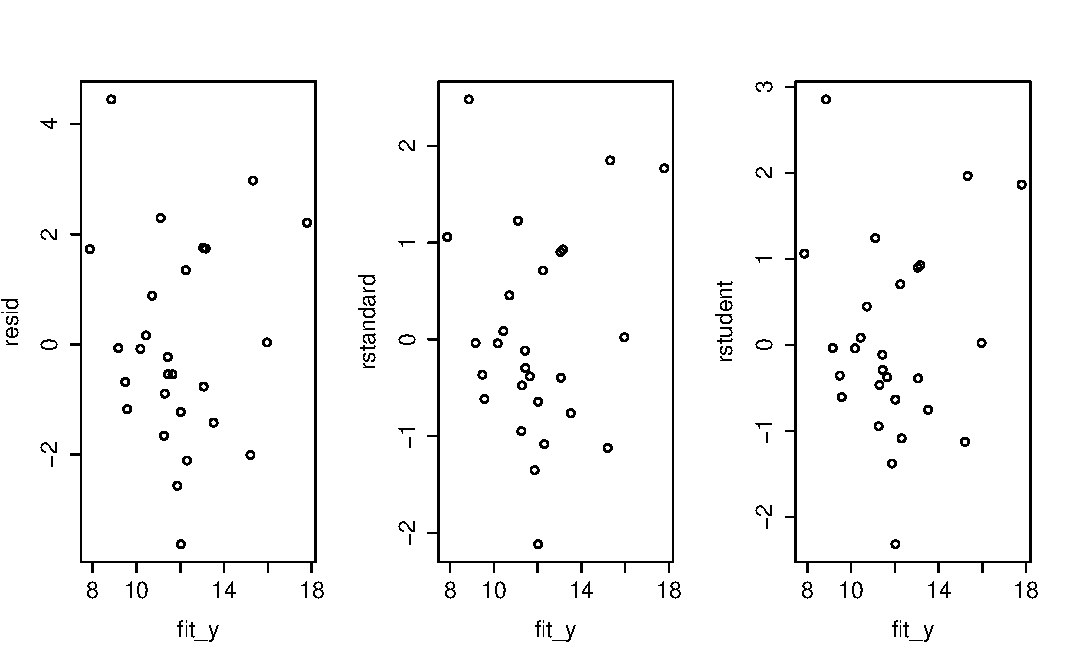
\includegraphics{figure/dy_残差比较}


\subsubsection{残差的正态性检验}

虽然从残差的QQ图中可以看出残差基本符合正太分布。但仍需在统计学上证其符合正态分布。

Shapiro-Wilk检验就是用来检验数据是否符合正态分布。该检验原假设为$H_{0}$:数据集符合正态分布,统计量W为:$W=\frac{\sum a_{i}y_{i}^{2}}{\sum(y_{i}-\bar{y})^{2}}$统计量越大则表示数据越符合正态分布,但是仅凭这一个参数是不够的,在非正态分布的小样本数据中也经常会出现较大的W值。通过R语言计算得最小二乘法回归的残差的W=0.9783,虽然W值小(接近于0),但p-value
= 0.8233,我们我们不能拒绝原假设,残差的确符合正态分布。


\subsubsection{多重共线性的诊断 }

设$x_{1},x_{2},\cdots,x_{m}$是自变量$X_{1},X_{2},\cdots,X_{m}$经过中心化和标准化得到的向量,记$x=(x_{1},x_{2},\cdots,x_{m})$,设$\lambda$为$X^{T}X$的一个特征值,$\varphi$为对应的特征向量,其长度为1,即$\varphi^{T}\varphi=1$若$\lambda\approx0$,则$x^{T}x\varphi=\lambda\varphi\approx0$,用$\varphi^{T}$左乘可到$\varphi x^{T}x\varphi=\varphi^{T}\lambda\varphi=\lambda\approx0$,所以有$x\varphi\approx0$,即$\varphi_{1}x_{1}+\varphi_{2}x_{2}+\cdots+\varphi_{m}x_{m}\approx0$,所以对应自变量$X_{1},X_{2},\cdots,X_{m}$,存在$c_{1},c_{2},\cdots,c_{m}$使得左式近似成立,即自变量之间存在着多重共线性。度量多重共线性严重程度的一个重要指标是矩阵$X^{T}X$的条件数,即$\kappa(X^{T}X)=||X^{T}X||\cdot||(X^{T}X)^{-1}||=\frac{\lambda_{max}(X^{T}X)}{\lambda_{min}(X^{T}X)}$

其中\foreignlanguage{english}{$\lambda_{max}(X^{T}X)$,$\lambda_{min}(X^{T}X)$分别表示矩阵$X^{T}X$的最大最小特征值。从实际应用的经验角度,一般若$\kappa$<100,则认为多重共线性的程度很小;若$100\leq\kappa\leq1000$,则认为存在中等程度或较强的多重共线性;若$\kappa$>1000,则认为存在严重的多重共线性。}

\selectlanguage{english}%
利用R语言得到条件数$\kappa$=11.42798,认为多重共线性的程度很小。

另一种常见的度量多重共线性严重程度的一个重要指标是方程膨胀因子(vif),通过R语言计算得:

\begin{tabular}{|c|c|c|c|c|}
\hline 
系数 & $\hat{\beta_{1}}$ & $\hat{\beta_{2}}$ & $\hat{\beta_{3}}$ & $\hat{\beta_{4}}$\tabularnewline
\hline 
\hline 
vif & 2.1855 & 1.7799 & 1.2784 & 1.2667\tabularnewline
\hline 
\end{tabular}

一般vif大于10或$\sqrt{vif_{i}}>2$说明存在这变量可能与其他变量存在复共线性,而从上面的数值可以看出,可以认为\foreignlanguage{english}{多重共线性的程度很小。}


\section{其他多元回归模型}


\subsection{岭回归(ridge regression)}

岭回归(ridge regression)可以用来处理下面两类问题:一是数据点少于变量个数;二是变量间存在共线性。

在最小二乘法中,当X列满秩时,有$\hat{\beta}=\left(X^{T}X\right)^{-1}X^{T}Y$.当X不是列满秩,或者某些某些列之间的线性相关性比较大时,$X^{T}X$的行列式接近于0,即$X^{T}X$接近于奇异,计算$\left(X^{T}X\right)^{-1}$时误差会很大。此时传统的最小二乘法缺乏稳定性与可靠性。

岭回归是对最小二乘回归的一种补充,它损失了无偏性,来换取高的数值稳定性,从而得到较高的计算精度。当$X^{T}X$的行列式接近于0时,我们将其主对角元素都加上一个数k,可以使矩阵为奇异的风险大降低。于是:$\hat{\beta}=\left(X^{T}X+kI\right)^{-1}X^{T}Y$.(I是单位矩阵)

随着k的增大,B(k)中各元素bi(k)的绝对值均趋于不断变小,它们相对于正确值bi的偏差也越来越大。k趋于无穷大时,B(k)趋于0。b(k)随k的改变而变化的轨迹,就称为岭迹。实际计算中可选非常多的k值,做出一个岭迹图,看看这个图在取哪个值的时候变稳定了,那就确定k值了。

在R语言中,MASS包中的函数lm.ridge()可以很方便的完成岭回归,通过计算得到k值为8.83。岭迹图如下所示:

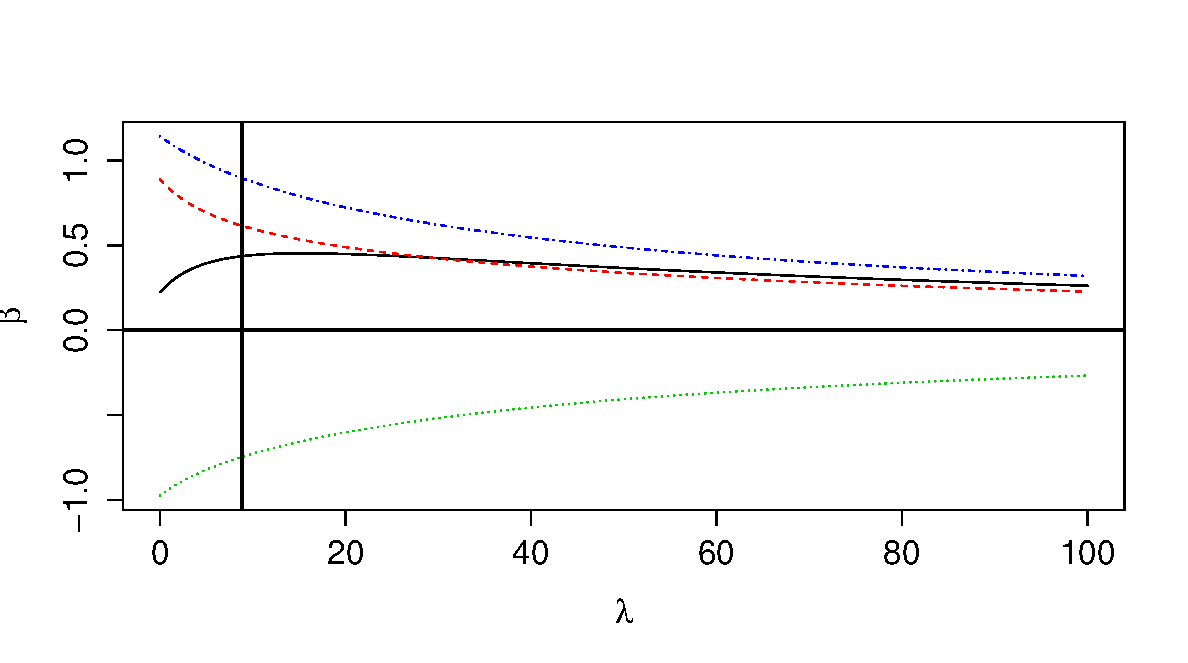
\includegraphics{figure/岭迹图}

有R语言分析得,bi(k)的绝对值在k=8.83的时候变稳定了,对应的系数如下表所示:

\begin{tabular}{|c|c|c|c|c|}
\hline 
 & $\hat{\beta_{1}}$ & $\hat{\beta_{2}}$ & $\hat{\beta_{3}}$ & $\hat{\beta_{4}}$\tabularnewline
\hline 
\hline 
OLS & 0.223 & 0.888 & -0.975 & 1.142\tabularnewline
\hline 
岭回归 & 0.436 & 0.615 &  -0.747  & 0.896\tabularnewline
\hline 
\end{tabular}


\subsection{主成分分析(principal components analysis, PCA)}

X不满足列满秩,换句话就是说样本向量之间具有高度的相关性(如果每一列是一个向量的话)。遇到列向量相关的情形,岭回归是一种处理方法,也可以用主成分分析PCA来进行降维。

主成分分析(principal components analysis, PCA)是一种分析、简化数据集的技术。它把原始数据变换到一个新的坐标系统中,使得任何数据投影的第一大方差在第一个坐标(称为第一主成分)上,第二大方差在第二个坐标(第二主成分)上,依次类推。主成分分析经常用减少数据集的维数,同时保持数据集的对方差贡献最大的特征。

设X是p维随机变量,病假设$\mu=E(x)$,$\Sigma=Var(X)$。并考虑如下线性变换$\begin{cases}
Z_{1}=a_{1}^{T}X\\
Z_{2}=a_{2}^{T}X\\
\vdots\\
Z_{p}=a_{p}^{T}X
\end{cases}$

$Var(Z_{i})=a_{i}^{T}\Sigma a_{i}$,$i=1,2,\cdots,p$,$Cov(Z_{i},Z_{j})=a_{i}^{T}\Sigma a_{j}$,$i,j=1,2,\cdots,p,i\neq j$.为使$Z_{1}$方差达到最大,即$a_{1}$是约束优化问题

$max\: a^{T}\Sigma a$

$s.t.\: a^{Ta}=1$

的解。

一般情况,对于协方差阵$\Sigma$,可由正交阵Q将其化为对角阵,即

$Q^{T}\Sigma Q=\left[\begin{array}{cccc}
\lambda_{1}\\
 & \lambda_{2}\\
 &  & \ddots\\
 &  &  & \lambda_{p}
\end{array}\right]$,且$\lambda_{1}>\lambda_{2}>\cdots>\lambda_{p}$。

则Q的第i列就对应于$a_{i}$,相应的$Z_{i}$为第i主成分。

R语言中进行主成分分析可以采用基本的princomp函数,将结果输入到summary和plot函数中可分别得到分析结果和碎石图。

碎石图如下图所示。 

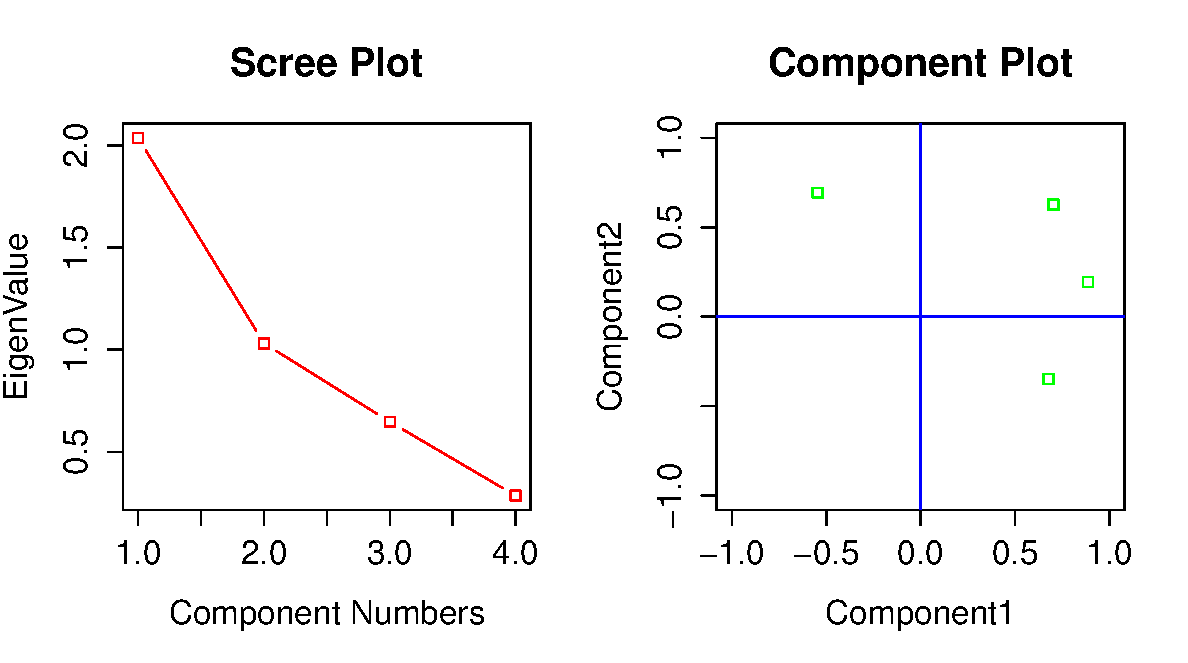
\includegraphics{figure/碎石图}

各成分的载荷矩阵为:

\begin{tabular}{|c|c|c|c|c|}
\hline 
 & Comp.1 & Comp.2 & Comp.3 & Comp.4\tabularnewline
\hline 
\hline 
$X_{1}$ & -0.621 & -0.191 & -0.18 & 0.738\tabularnewline
\hline 
$X_{2}$ & -0.493 & -0.617 & -0.115 & -0.602\tabularnewline
\hline 
$X_{3}$ & 0.382 & -0.682 & 0.556 & 0.281\tabularnewline
\hline 
$X_{4}$ & -0.475 & 0.342 & 0.803 & -0.115\tabularnewline
\hline 
\end{tabular}

每个变量在因子向量中的载荷图如下所示(未作因子旋转):

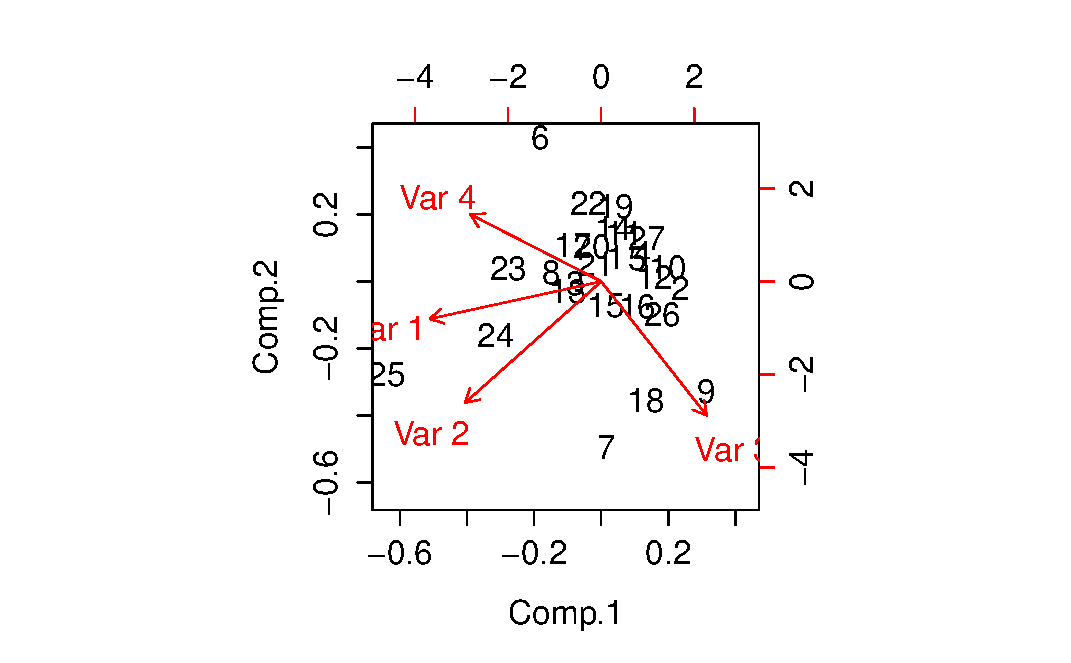
\includegraphics[scale=0.5]{figure/bio_载荷}

分析结果如下表:

\begin{tabular}{|c|c|c|c|c|}
\hline 
 & Comp.1 & Comp.2 & Comp.3 & Comp.4\tabularnewline
\hline 
\hline 
Standard deviation & 1.4270707 & 1.0154272 & 0.8043559 & 0.53421759\tabularnewline
\hline 
Proportion of Variance & 0.5091327 & 0.2577731 & 0.1617471 & 0.07134711\tabularnewline
\hline 
Cumulative Proportion & 0.5091327 & 0.7669058 & 0.9286529 & 1\tabularnewline
\hline 
\end{tabular}

从上图和表中可以看出,前2个主成分的累计贡献率达到76.6\%,前2个主成分的累计贡献率达到92.8\%。所以可以舍去最后1个或最后2个主成分,达到降维的目的。

所以,可以舍去最后1个成分,用前3个成分做回归,得:$\hat{Y}=11.9259-1.4903Z_{1}+0.4645Z_{2}+0.2327Z_{3}$,其中$Z_{1},Z_{2},Z_{3}$是前3个主成分。把3个主成分的表达式$Z_{1}=-0.621X_{1}-0.493X_{2}+0.382X_{3}-X_{4}$,$Z_{2}=-0.1911X_{1}-0.617X_{2}-0.682X_{3}+0.342X_{4}$
,$Z_{3}=-0.18X_{1}-0.115X_{2}+0.556X_{3}-0.803X_{4}$代入到回归表达式易得:

$\hat{Y}=11.9259+0.7953X_{2}+0.4211X_{2}-0.7567X_{3}+1.0528X_{4}$将其与原最小二乘法得到的回归方程$\hat{Y}=5.9433+0.1424X_{1}+0.3515X_{2}-0.2706X_{3}+0.6382X_{4}$比较发现,只选取3个主成分做的回归虽然系数与最小二乘法得到回归方程的系数的不同,但系数的符号没有变化,系数的大小差距比较小。由此我们可以的得出,在适当的条件下,可以由主成分回归方程代替最小二乘回归方程。


\section{总结 }

本文由问题引入,简单介绍多元线性回归模型及其参数的求解,然后用多元线性回归模型来测算糖尿病患者的血清总胆固醇、甘油三酯、空腹胰岛素、糖化血红蛋白和空腹血糖的测量值之间的关系,得到回归方程为:$\hat{Y}=5.9433+0.1424X_{1}+0.3515X_{2}-0.2706X_{3}+0.6382X_{4}$。从各项系数都为正数可知,糖尿病患者的血清总胆固醇、甘油三酯、空腹胰岛素、糖化血红蛋白都对空腹血糖有着正相关关系,即在其他情况不变的条件下,它们中任何一个升高,对应的平均血糖也会升高。然后进行了方差分析,根据F检验求得的统计量确定所建的回归方程具有统计学意义。而且回归模型的$R^{2}=0.6008$,表明糖尿病患者血糖含量变异的60\%可以由总胆固醇、甘油三酯、胰岛素和糖化血红蛋白的变化来解释。虽然$R^{2}=0.6008$说明模型拟合结果较好,但仍希望能进一步提高拟合效果。于是做了t检验分析各项回归系数的显著性,发现只有$\hat{\beta_{3}}$和$\hat{\beta_{4}}$显著异于零,即糖尿病患者的血糖含量的确受到空腹胰岛素($X_{3}$)、糖化血红蛋白($X_{4}$)的影响。又进一步求了回归系数的置信区间,从置信区间看出$\hat{\beta_{3}}$和$\hat{\beta_{4}}$的置信区间不包含0,而$\hat{\beta_{1}}$和$\hat{\beta_{2}}$的置信区间包含0,说明在置信度区间内,$\hat{\beta_{1}}$和$\hat{\beta_{2}}$可能取值为0,即糖尿病患者的血糖含量可能不受血清总胆固醇、甘油三酯的影响。为比较各项变量对因变量的影响,由标准化回归方程和偏回归平方和可以看出,对血糖影响大小的顺序依次为糖化血红蛋白($X_{4}$)、
胰岛素($X_{3}$)、 甘油三脂 ($X_{2}$)和总胆固醇($X_{1}$)。因为$\hat{\beta_{1}}$和$\hat{\beta_{2}}$系数不显著可能是受到其他变量的影响,因此又做了自变量的选择和是否存在交互作用的判断。

为判断回归模型时候有效,本文又比较了回归的残差并检验的残差的确符合正态分布,而且检验得回归的设计矩阵的多重共线性很小。为比较普通最小二乘法的效果,本文又比较了岭回归和主成分分析做出的回归方程。

在实际问题中,一种现象常常是与多个因素相联系的,由多个自变量的最优组合共同来预测或估计因变量,比只用一个自变量进行预测或估计更有效,更符合实际。因此多元线性回归应用地比一元线性回归更广。而且,多元回归分析还可以分析哪些因素有影响,哪些因素影响较大。多元回归分析虽然在多元回归方程中虽然很简单,但在大多数问题中十分使用。所以,掌握多元线性回归的应用与分析,具有很重要的实际意义。
\end{document}
